\chapter{Low-Level Control}

\section{Control Architecture}

During early prototyping, the low level controller for the motors was an Arduino Uno, based on the ATmega328P microcontroller. While this allows for swift validation, there were multiple disadvantages that made this inappropriate for final deployment. For one, this is an 8-bit RISC architecture, which means that for high step counts or floating-point mathematics, the CPU must perform multiple cycles of software-emulated mathematics because it cannot store the number. Moreover, since there is no hardware math co-processor, every calculation of a trigonometric function (required for S-curves) takes hundreds of clock cycles, which will cause issues in synchronization in the pulse train. And since the Arduino communicates with the PC using Serial, the CPU must stop and wait for the text every time it is used. Considering the precision and timing requirements of the task at hand, these cons amalgamate into major concerns.

Hence, the project shifted to the STM32 ecosystem, particularly the STM32F303 Discovery Kit that was available in the University. There are many advantages of this architectural shift:

\begin{enumerate}
    \item The board uses the ARM Cortex-M4 core, which handles 32-bit integers in a single clock cycle. Hence, conversion of steps to distance, which can easily exceed the 16-bit integer limit (65535), can be completed without risking overflow errors.
    \item There is a Hardware Floating Point Unit (FPU) present, which can calculate transcendental functions (such as sine and cosine) for S-curve profiles in a fraction of the time required on the ATmega328P, so that time between pulses can remain consistent and operation of motors smooth.
    \item The STM32 has a Nested Vectored Interrupt Controller (NVIC), which essentially allows priorities to be set to interrupts. For example, the limit switch interrupt can be set to the highest priority, so that there would be no delay in responding to an axis hitting a limit, no matter what task the CPU is busy with. 
    \item There is useful variety in timers, with features such as Auto-Reload Registers and Prescalers. One example of a mode that can be utilized is Output Compare, where the pulse train can be generated entirely in hardware after timer configuration, so that the CPU does not need to toggle the pin manually. Hence, the processor is freed up to handle other tasks. For S-curves, though, the ARR/CRR register would need to be updated every time period since the inter-pulse interval changes every step.
    \item To address the blocking nature of Serial communication, the STM32 uses Direct Memory Access, where the UART can receive JSON commands and store them directly into a RAM buffer without CPU involvement, so that the STM32 does not experience lag in other critical tasks. The CPU still needs a flag to know when the entire JSON has arrived, but this is far less involvement than on an Arduino.
    \item Finally, the STM32 supports the usage of Real Time Operating Systems, particularly FreeRTOS, so that the firmware can be split into high-priority and low-priority tasks, which allows for more sophisticated management and allocation of resources to accomplishing low-level control.
\end{enumerate}

\section{Drive Interfacing}

The STM32 interfaces with the SGDV drive using a pulse/direction protocol, similar to commanding a stepper motor. Each rising edge on the PULS pin increments an internal counter on the drive by one, or decrements if SIGN is LOW (opposite direction). With this information, the control loop drives the shaft until the encoder feedback confirms that the shaft has reached the intended position.

However, the motor encoder has a 20-bit resolution corresponding to $2^{20}$ = 1048576 counts per revolution, which is an awkward number for firmware mathematics. Hence, the drive has an electronic gear ratio parameter, where registers Pn20E is set to 1048576 and Pn210 to 10000, so that one full revolution is exactly 10000 pulses. Each pulse therefore commands $\approx 104.86$ encoder counts of shaft displacement. This has been experimentally verified on the test bench by sending exactly 10000 pulses and visually confirming a single motor revolution on the motor shaft, as well as reading the number of pulses received on the drive itself.

Table~\ref{tab:cn1_wiring} summarizes the CN1 pin – the connector that allows interfacing with a microcontroller -- assignments used in this project. \begin{table}[h] \centering \caption{Yaskawa SGDV CN1 Wiring Summary} \label{tab:cn1_wiring} \begin{tabular}{|c|l|l|l|} \hline \textbf{Pin} & \textbf{Signal} & \textbf{Connection} & \textbf{Function} \\ \hline 47 & +24VIN & +24V PSU & Sequence input common power \\ 42 & P-OT & 24V PSU GND & Bypass forward overtravel limit \\ 43 & N-OT & 24V PSU GND & Bypass reverse overtravel limit \\ 40 & /S-ON & MCU GPIO & Active-low drive enable \\ 7 & PULS & MCU GPIO / AM26LS31 & Step pulse command \\ 8 & /PULS & MCU GND / AM26LS31 & Step pulse return / complement \\ 11 & SIGN & MCU GPIO / AM26LS31 & Direction command \\ 12 & /SIGN & MCU GND / AM26LS31 & Direction return / complement \\ \hline \end{tabular} \end{table}

During prototyping, an open-collector topology was employed, where the current path starts from the MCU pin, goes through a resistor and into the CN1 optocoupler. Because of this, grounding is critical, as if the MCU ground and 24V PSU ground are at slightly different potentials, then the current flowing through the optocoupler is no longer reliable due to losing predictability. With grounding, an MCU’s GPIO LOW being drawn to 0V is the same reference as the cathode return path of the optocoupler.

While this worked, this is not the best choice for industry deployment, because this signal is single-ended; that is, there is only one wire whose voltage is measured relative to ground. Hence, if any noise occurs in the signal – particularly from electromagnetic interference from the power wires nearby – the receiver can no longer distinguish between it and the genuine signal. This noise grows with pulse rate and long cable runs, which will be experienced in the final deployment, so open-collector topology can eventually lead to poor position control.

To address this, the solution implements a differential line driver, where two wires send inverted signals. For example, if the signal is a +3.3V/0V differential and experiences +0.5V noise on both from electromagnetic interference, then the difference between the wires is unaffected and remains to be 3.3V. This is known as common-mode rejection, since the noise is experienced by both wires and hence is cancelled out through subtraction. For this to function, the noise needs to affect both wires equally, which is why the wires need to be twisted to see nearly identical electromagnetic environments along the cable. To address this, the solution utilizes shielded twisted pair cabling for the PULS and SIGN pins.

This topology has another advantage. Open-collector topology is passive, so it can only pull the line low, which leads to a weak drive strength for pulling high and therefore susceptibility to parasitic capacitance. In contrast, the differential line driver is active, so it pushes the line to high and pulls to low with controlled output impedance; no matter how long the cable is, the driver ensures sharp and fast edges.

Finally, within differential line driver topology, there are multiple input pulse modes supported by the SGDV, each with different trade-offs in complexity and noise immunity.

\begin{enumerate}

\item Sign + pulse mode. Here, one pair sends a pulse train corresponding to position increments, while the other pair simply sends a HIGH or LOW depending on the direction. This is simple to generate and debug, but needs settling time for changing direction before issuing the next pulse.
\item Clockwise + Counter-Clockwise, where only one pair sends a pulse train at a time, of which one pair corresponds to forward motion (clockwise), and one pair backward (counter-clockwise). There is no settling time for direction, but is more complex and has undefined behavior when both pairs send pulse trains.
\item Quadrature (2-phase), where both pairs send signals, 90 degrees out of phase. The direction is decided depending on which pair is leading. This quadruples the resolution, since now rising and falling edges can be counter on both pairs, and is highly immune to noise. However, this is non-trivial to generate, and is normally utilized on proprietary hardware.
\end{enumerate}
Considering the use case, the solution selects sign + pulse mode, as the required pulse rate is relatively low, and shielded twisted cabling addresses concerns of noise immunity.

\section{Command Trajectory}

The SGDV has an internal feedback control system with auto-tuned PID parameters, so that the torque can be controlled to correct position error. However, the command it receives cannot be smoothened, so if a rapid succession of pulses is received, then the drive sees an immediate and enormous position error, so it demands maximum torque instantaneously. This can lead to mechanical shock and significant vibration, which in turn can cause faults (most notably the A.d00 following error fault) and wear on the belt/rack. 

Thus, distinct from the PID, the solution requires a motion profile. In particular, the command trajectory needs its acceleration and jerk to be continuous, so that transitions can be smoother. One rudimentary example is the trapezoidal profile, where the velocity graph follows a trapezoidal shape. While this is better than a step input, this means that the acceleration graph has sudden jumps at the corners, which leads to infinite jerk. For the project, this is insufficient.

To ensure a finite and controlled jerk, a known method is the S-curve. Here, the acceleration itself is ramped, so that the velocity follows a smooth S-shape instead of straight lines, and the acceleration graph itself becomes continuous. As a result, jerk is now finite and controlled.

The STM32, in the project's case, approximates this using a sinusoidal ease function. The equation is:
\begin{equation}
    t = \frac{i}{N_{accel}}, \tilde{t} = \frac{1}{2}(1-\cos{(\pi t)}) 
\end{equation}

where $i$ is the current step index inside the acceleration region, $N_{accel}$ is the total number of acceleration steps, $t$ is the normalized linear progress through the ramp (akin to time), and $\tilde{t}$ is the shaped version. 

The cosine is a good option for the S-curve because it naturally starts at 1 and ends at -1, with a smooth S-shaped profile in between 0 and $\pi$. After the transformation defined in the equation, this goes from 0 to 1, which is what is required. And more importantly, the rate of change of $\tilde{t}$ is 0 at the beginning and end of the ramp, so there is zero jerk at the transitions.

Then the delay  interpolation:
\begin{equation}
    d(i) = d_{min}+(d_{max}-d_{min})(1-\tilde{t})
\end{equation}
where $d_{min}$ is the slow delay and $d_{max}$ is the maximum delay; since delay is inversely proportional to velocity (time between pulses decreases leading to faster movement), $\tilde{t}=0$ gives minimum speed and $\tilde{t}=1$ gives maximum speed. 

Now, there are three regions in the S-curve: acceleration, cruise, and deceleration. Deceleration mirrors acceleration by indexing from the end of the move instead of the beginning, which creates a constraint. If the acceleration region were longer than half the graph, it would overlap with the deceleration region, which is geometrically impossible within the available steps. Because of this, the acceleration length needs to be capped at half the total step count. Meanwhile, the cruise region has no acceleration, so the delay value is now constant and the velocity curve is flat.

This discussion, so far, has focused on a single axis. For simultaneous multi-axis movement, all axes must share a single delay curve depending on the axis with the greatest count of steps. What this means is that if one axis needs to move 1000 steps and another 500 steps, then to ensure that they start and stop together in, say, 1000 iterations, the second axis must skip pulse opportunities relative to the dominant axis. This way, all axes reach the required positions simultaneously, and the end-effector can follow an approximately linear path.

Currently, this has been implemented on the Arduino prototype firmware, and will be migrated to the STM32, where the FPU can more efficiently compute the sinusoidal ease function in real-time. 
\begin{figure}[H]
    \centering
    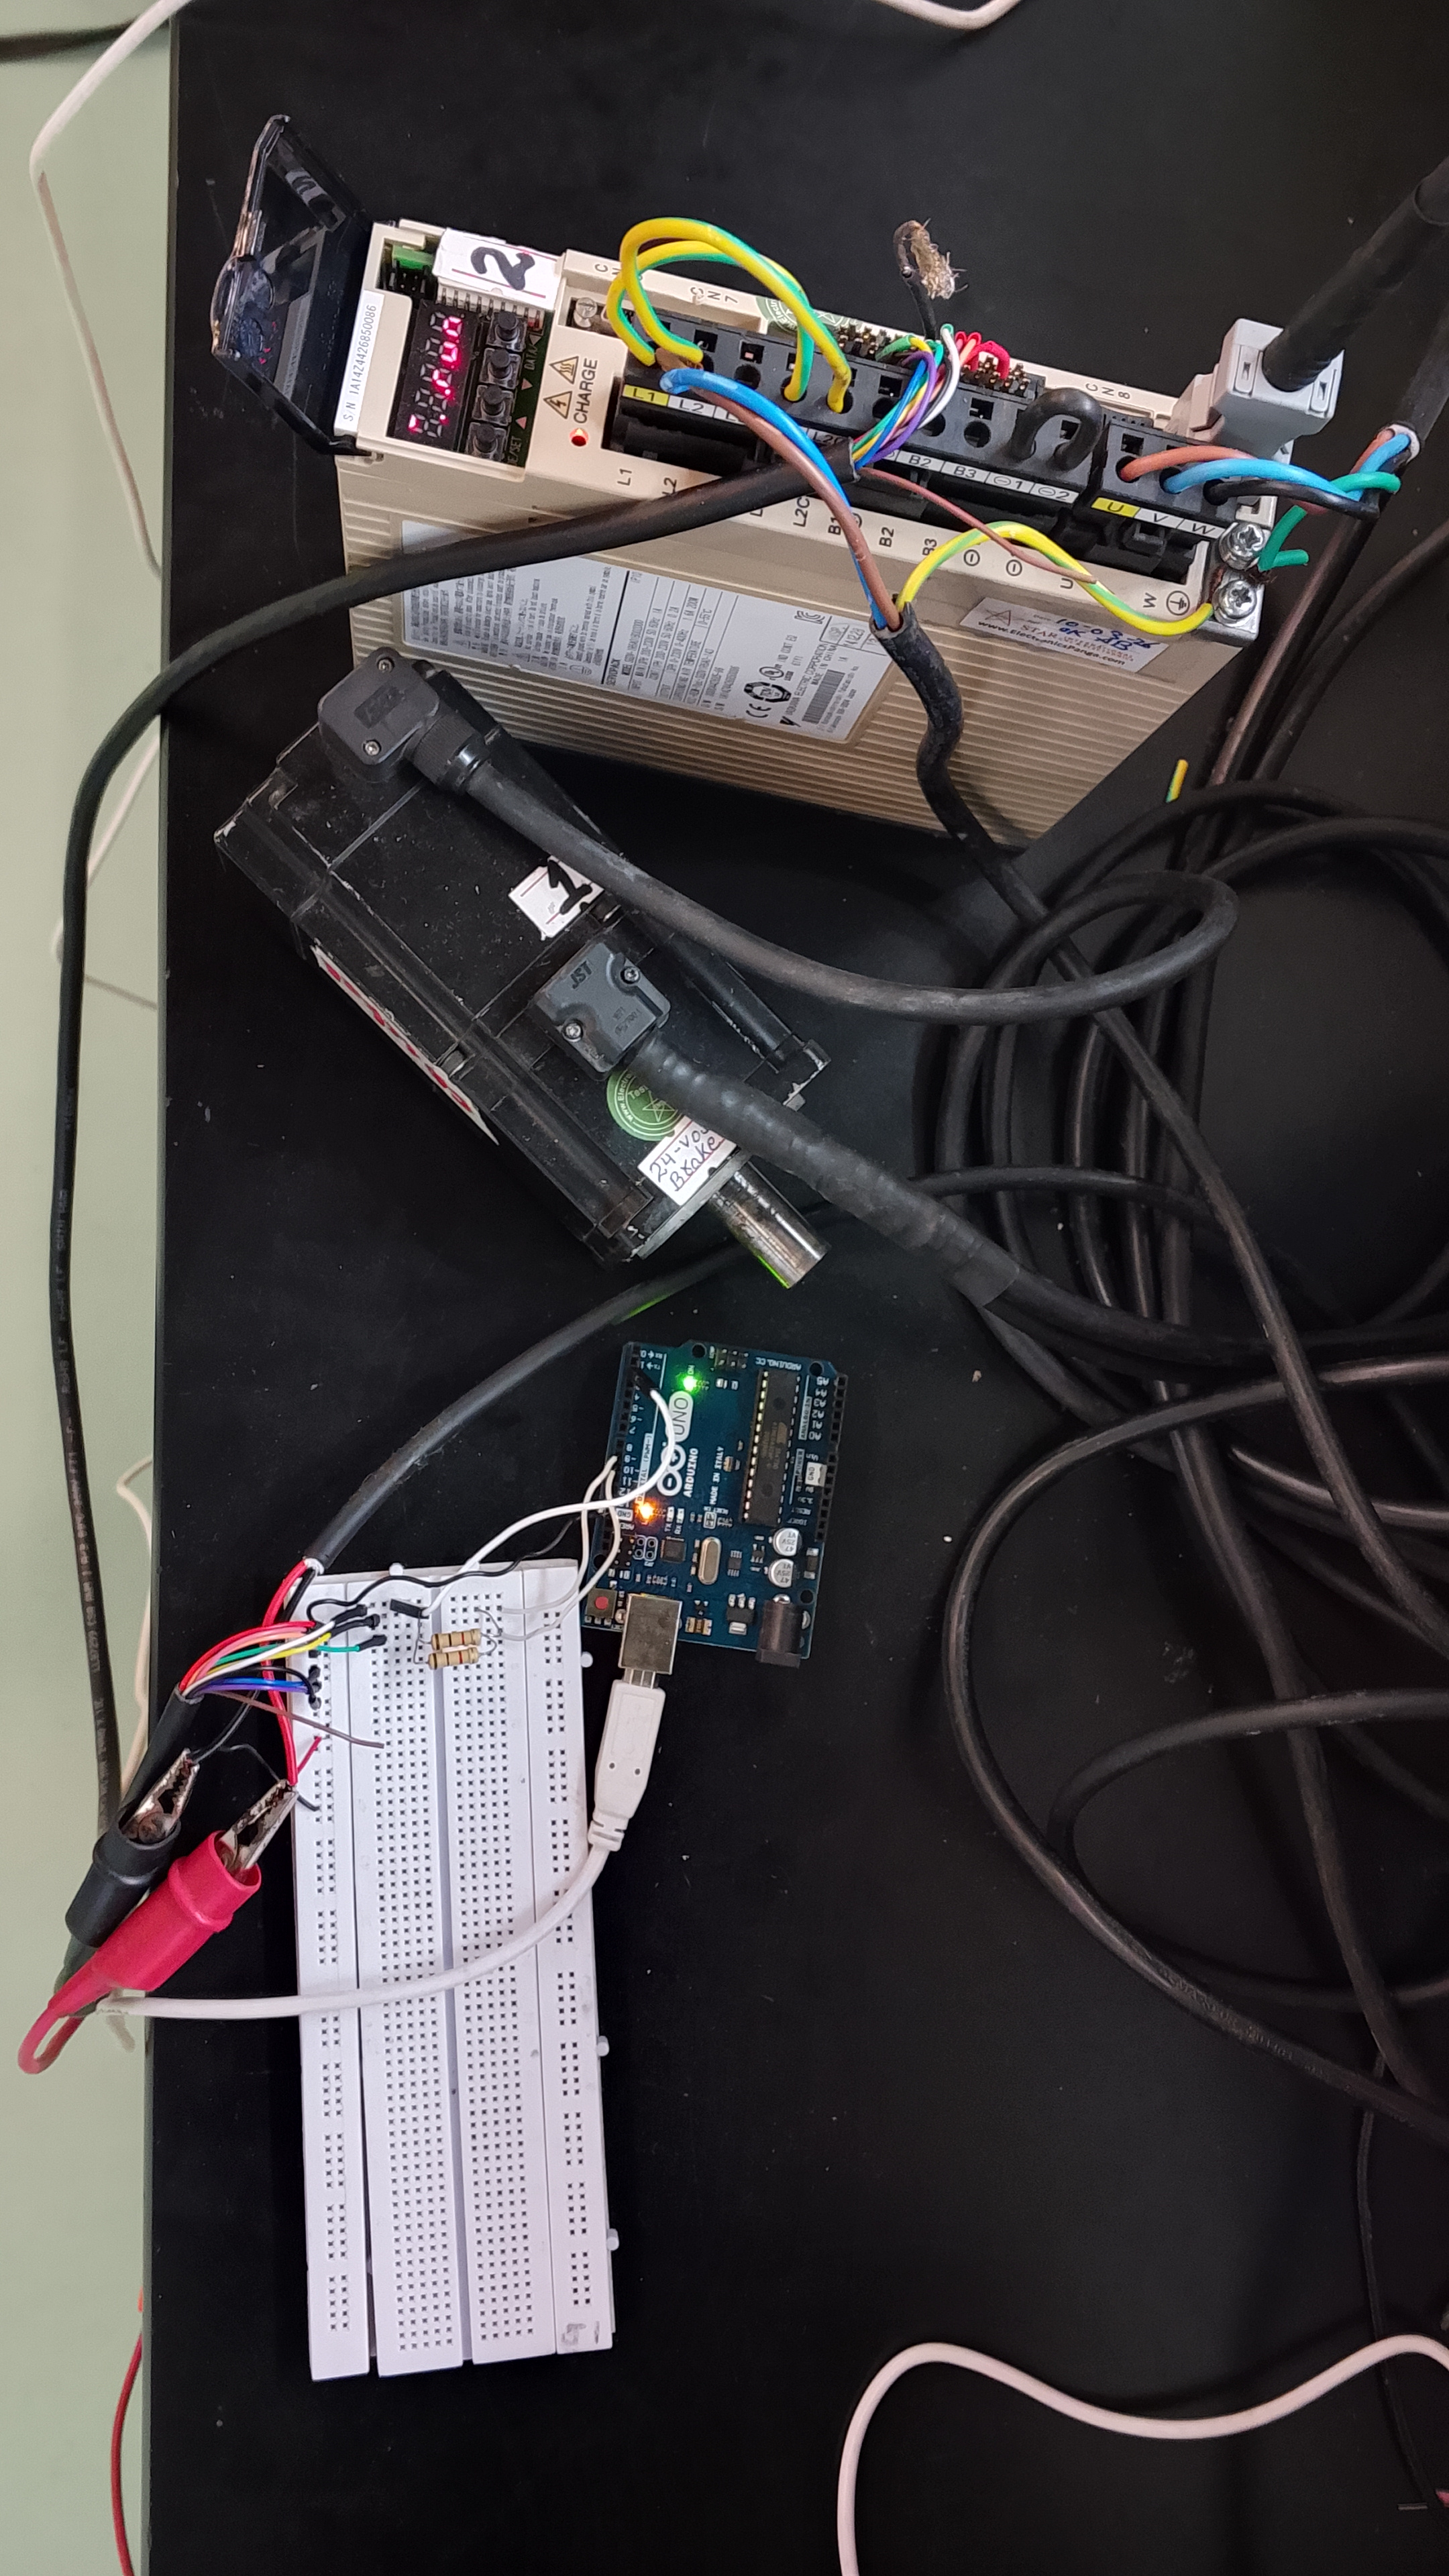
\includegraphics[width=0.6\linewidth]{motor_test_bench.jpeg}
    \caption{Motor test bench using the Arduino Uno.}
    \label{fig:placeholder}
\end{figure}

Moreover, a homing mechanism has been implemented in the X and Y-axes on the smaller wooden prototype using limit switches. The axis moves towards the switch at high speed until it triggers, after which is backs off slowly to release the trigger. The final location reached is the coordinate reference (home), so that all subsequent moves are relative to that known position.
% 1. Motivation (~2 paragraphs)

% Why infinite jerk is mechanically harmful — frame around your three consequences (shock/vibration, following error fault, mechanical wear)
% Why a motion profile solves this — the idea of shaping the command trajectory as distinct from the drive's PID

% 2. Profile Comparison (~1 paragraph)

% Trapezoidal: what it is, where jerk is still infinite (the corners), why it's insufficient
% S-curve: what it adds over trapezoidal — finite jerk, smooth acceleration transitions

% 3. Mathematical Implementation (~2 paragraphs)

% The sinusoidal ease function — write out the equation, explain what t and smoothT represent physically
% How smoothT maps to inter-pulse delay — the interpolation between minDelay and maxDelay, and why shorter delay = higher velocity

% 4. Acceleration Region Geometry (~1 paragraph)

% The three regions: accel, cruise, decel
% Why accel = min(accelSteps, maxSteps/2) — the overlap argument
% What accelSteps controls physically and consequences of tuning it too aggressively

% 5. Multi-Axis Coordination (~1 paragraph)

% How all axes share the same delay curve
% Why maxSteps drives the profile — the axis with most steps sets the pace
% What this achieves mechanically: all axes start and stop together